\documentclass[a4paper, 11pt]{report}
\usepackage{blindtext}
\usepackage[T1]{fontenc}
\usepackage[utf8]{inputenc}
\usepackage{titlesec}
\usepackage{fancyhdr}
\usepackage{geometry}
\usepackage{fix-cm}
\usepackage[hidelinks]{hyperref}
\usepackage{graphicx}
\usepackage{multirow}
\usepackage[english]{babel}
\usepackage{graphicx}
\usepackage{caption}

\geometry{ margin=30mm }
\counterwithin{subsection}{section}
\renewcommand\thesection{\arabic{section}.}
\renewcommand\thesubsection{\thesection\arabic{subsection}.}
\usepackage{tocloft}
\renewcommand{\cftchapleader}{\cftdotfill{\cftdotsep}}
\renewcommand{\cftsecleader}{\cftdotfill{\cftdotsep}}
\setlength{\cftsecindent}{2.2em}
\setlength{\cftsubsecindent}{4.2em}
\setlength{\cftsecnumwidth}{2em}
\setlength{\cftsubsecnumwidth}{2.5em}


\begin{document}
\titleformat{\section}
{\normalfont\fontsize{15}{0}\bfseries}{\thesection}{1em}{}
\titlespacing{\section}{0cm}{0.5cm}{0.15cm}
\titleformat{\subsection}
{\normalfont\fontsize{13}{0}\bfseries}{\thesubsection}{0.5em}{}
\titlespacing{\section}{0cm}{0.5cm}{0.15cm}

%=======================================================================================

% #########################
% IMPORTANT - Add student names here!
% e.g. \newcommand{\stud1}{LOWE, David}
\newcommand{\studA}{{Fan Kaffa}}
\newcommand{\studB}{{Lin Link}}
\newcommand{\studC}{{Song Jared}}
\newcommand{\studD}{{Zheng Barnett}}
% ADD ANOTHER LINE FOR A FIFTH MEMBER
%
% IMPORTANT - Then give your SIDs
\newcommand{\sidA}{{510041359}}
\newcommand{\sidB}{{540801400}}
\newcommand{\sidC}{{550155230}}
\newcommand{\sidD}{{550718806}}
% ADD ANOTHER LINE FOR A FIFTH MEMBER

%
% IMPORTANT - And then update which major each student will focus on
\newcommand{\majA}{{Computer Science}}
\newcommand{\majB}{{Data Science}}
\newcommand{\majC}{{SW Development}}
\newcommand{\majD}{{Cyber Security}}
% ADD ANOTHER LINE FOR A FIFTH MEMBER - HCI

% #########################


\pagenumbering{Alph}
\begin{titlepage}
\begin{flushright}

\includegraphics[width=4cm]{USyd}\\[1cm]
\end{flushright}

\begin{centering}
\textbf{\huge INFO1111: Computing 1A Professionalism}\\[0.75cm]
\textbf{\huge 2025 Semester 1}\\[2cm]
\textbf{\huge Skills: Team Project Report}\\[2cm]

\textbf{\large Submission number: T4 SL Group 6 (1)}\\[0.5cm]
{\large \textbf{Github link: \url{https://github.com/KaltsitFan/INFO1111_GROUP.git}}}\\[0.75cm]
\textbf{\huge Team Members:}\\[0.75cm]

\begin{tabular}{|p{0.25\textwidth}|p{0.13\textwidth}|p{0.12\textwidth}|p{0.12\textwidth}|p{0.22\textwidth}|}
	\hline
	\multirow{2}{*}{Name} & \multirow{2}{*}{Student ID} & Target * & Target * & \multirow{2}{*}{Selected Major} \\
	 & & Foundation & Advanced & \\
	\hline
	\hline
	\raggedright{\studA} & \sidA & A & NA & Computer Science \\
	\hline
	\raggedright{\studB} & \sidB & A & NA & \majB \\
	\hline
	\raggedright{\studC} & \sidC & A & NA & \majC \\
	\hline
	\raggedright{\studD} & \sidD & A & NA & \majD \\
	\hline
\end{tabular}
\\[0.5cm]
\end{centering}

* Use the following codes:
\begin{itemize}
\setlength\itemsep{0em}
\item NA = Not attempting in this submission
\item A = Attempting (not previously attempting)
\item AW = Attempting (achieved weak in a previous submission) 
\item AG = Attempting (achieved good in a previous submission)
\item S = Already achieved strong in a previous submission
\end{itemize}

\thispagestyle{empty}
\end{titlepage}
\pagenumbering{arabic}


%=======================================================================================

\tableofcontents

%=======================================================================================
\newpage

\section{Group Response}

\newpage
\section{Individual Response}

\subsection{Skills for Computer Science: Kaffa Fan }
\section*{Personal Skill Reflection (Computer Science)}

In the disaster response system project, my primary responsibilities included the establishment of the overall system architecture, the setup of the GitHub collaboration framework, and the configuration of the LaTeX documentation environment. Reflecting based on the SFIA framework, I selected the following two skills:

\subsection*{1. Software Development (PROG)}

According to the SFIA framework~\cite{sfia}, software development is foundational to implementing various technological solutions within the computer science domain. Mastery of LaTeX as a report-writing tool requires proficiency in real-time debugging and structured document organization.
\textbf{Skill Enhancement (Team Collaboration Details):}

Initially, I decided that the team would use a plain text editor to write LaTeX code because most of my teammates had not installed any latex environments. And Unlike Overleaf, these editors lacked real-time output previews, leading to frequent errors, such as missing commands like \texttt{\textbackslash end\{itemize\}}, resulting in significant debugging time.

Later, by transitioning to Visual Studio Code (VS Code) and installing plugins like LaTeX Workshop and LaTeX Language Support, we enabled real-time compilation and error notifications. This substantially improved coding efficiency and code quality.

\textbf{Areas for Further Improvement:}

Currently, there is an over-reliance on real-time feedback from development tools. Moving forward, I aim to strengthen my proactive code review and logical self-checking skills to enhance code robustness.

\subsection*{2. Systems Integration and Build (SINT)}

According to the SFIA framework~\cite{sfia}, systems integration and build skills emphasize efficient integration of various modules to ensure smooth operation of the final system.
\textbf{Skill Enhancement (Team Collaboration Details):}

Initially, communication barriers existed within our team due to different personal communication habits. This caused vague task allocation and reduced efficiency.

To address these communication issues, the team adopted GitHub Issues for clear task division and tracking. Tasks such as "Frontend Interface Design" and "Data Interface Development" were specifically defined, allowing team members to clearly understand and take responsibility for their respective areas.

\textbf{Areas for Further Improvement:}

Technical discussions still contained excessive professional jargon, and unfamiliarity with various software and environments led to difficulties in comprehension among other team members. In the future, I should enhance my ability to explain complex technical concepts in simpler terms to improve cross-disciplinary communication effectiveness.

\section*{3. Git Response}

\textbf{1. Clone the repository}
\begin{verbatim}
git clone https://github.com/KaltsitFan/INFO1111_T4_SL_GROUP_6
\end{verbatim}
Download a copy of the remote repository to your local computer.This picture is show clone

\begin{center}
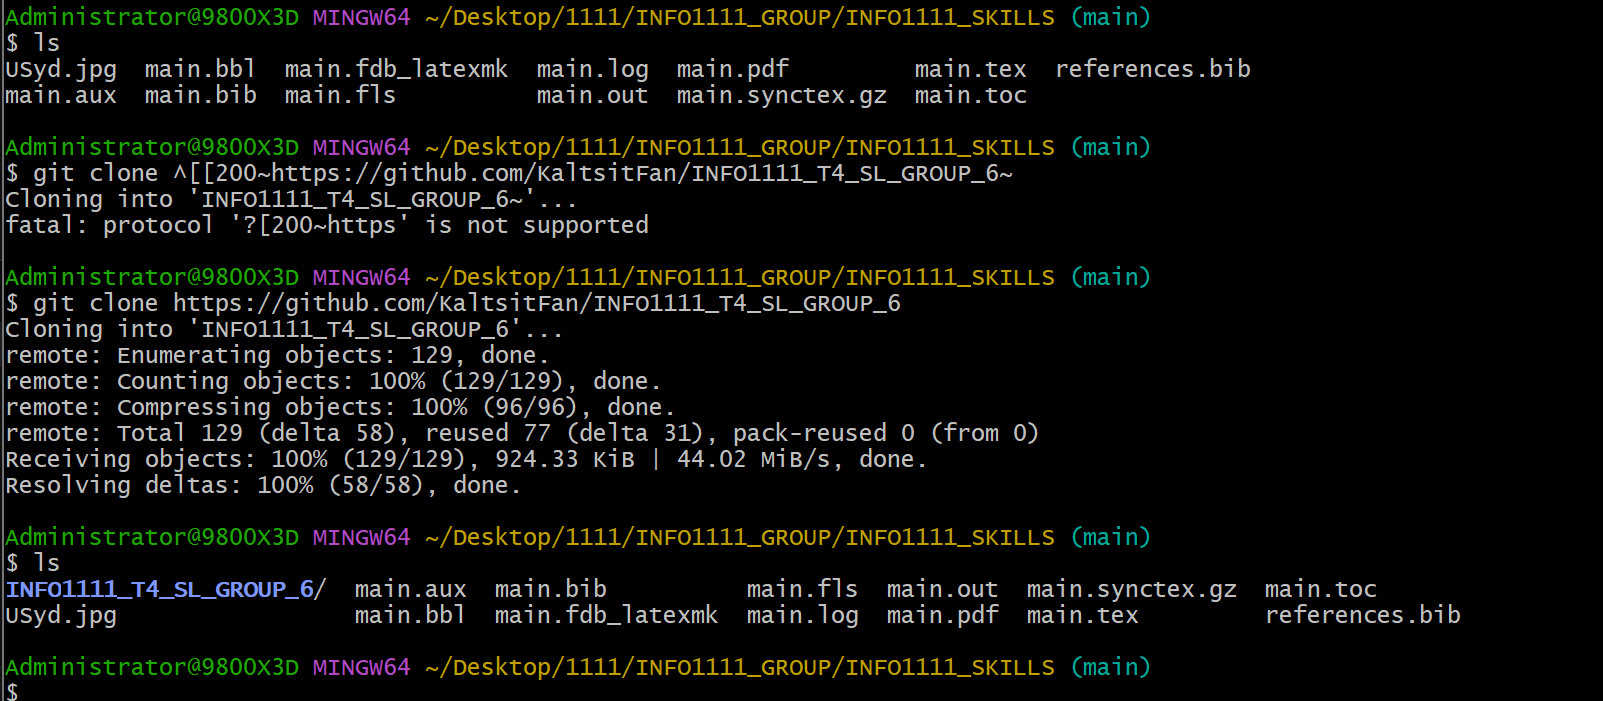
\includegraphics[width=0.8\textwidth]{kaffa/clone.png}
\captionof{figure}{Cloning the repository}
\end{center}

\textbf{2. Add all changed files}
\begin{verbatim}
git add ./ git comimt -m"" / git push / git status
\end{verbatim}
Stage all modified files to prepare them for commit.

\begin{center}
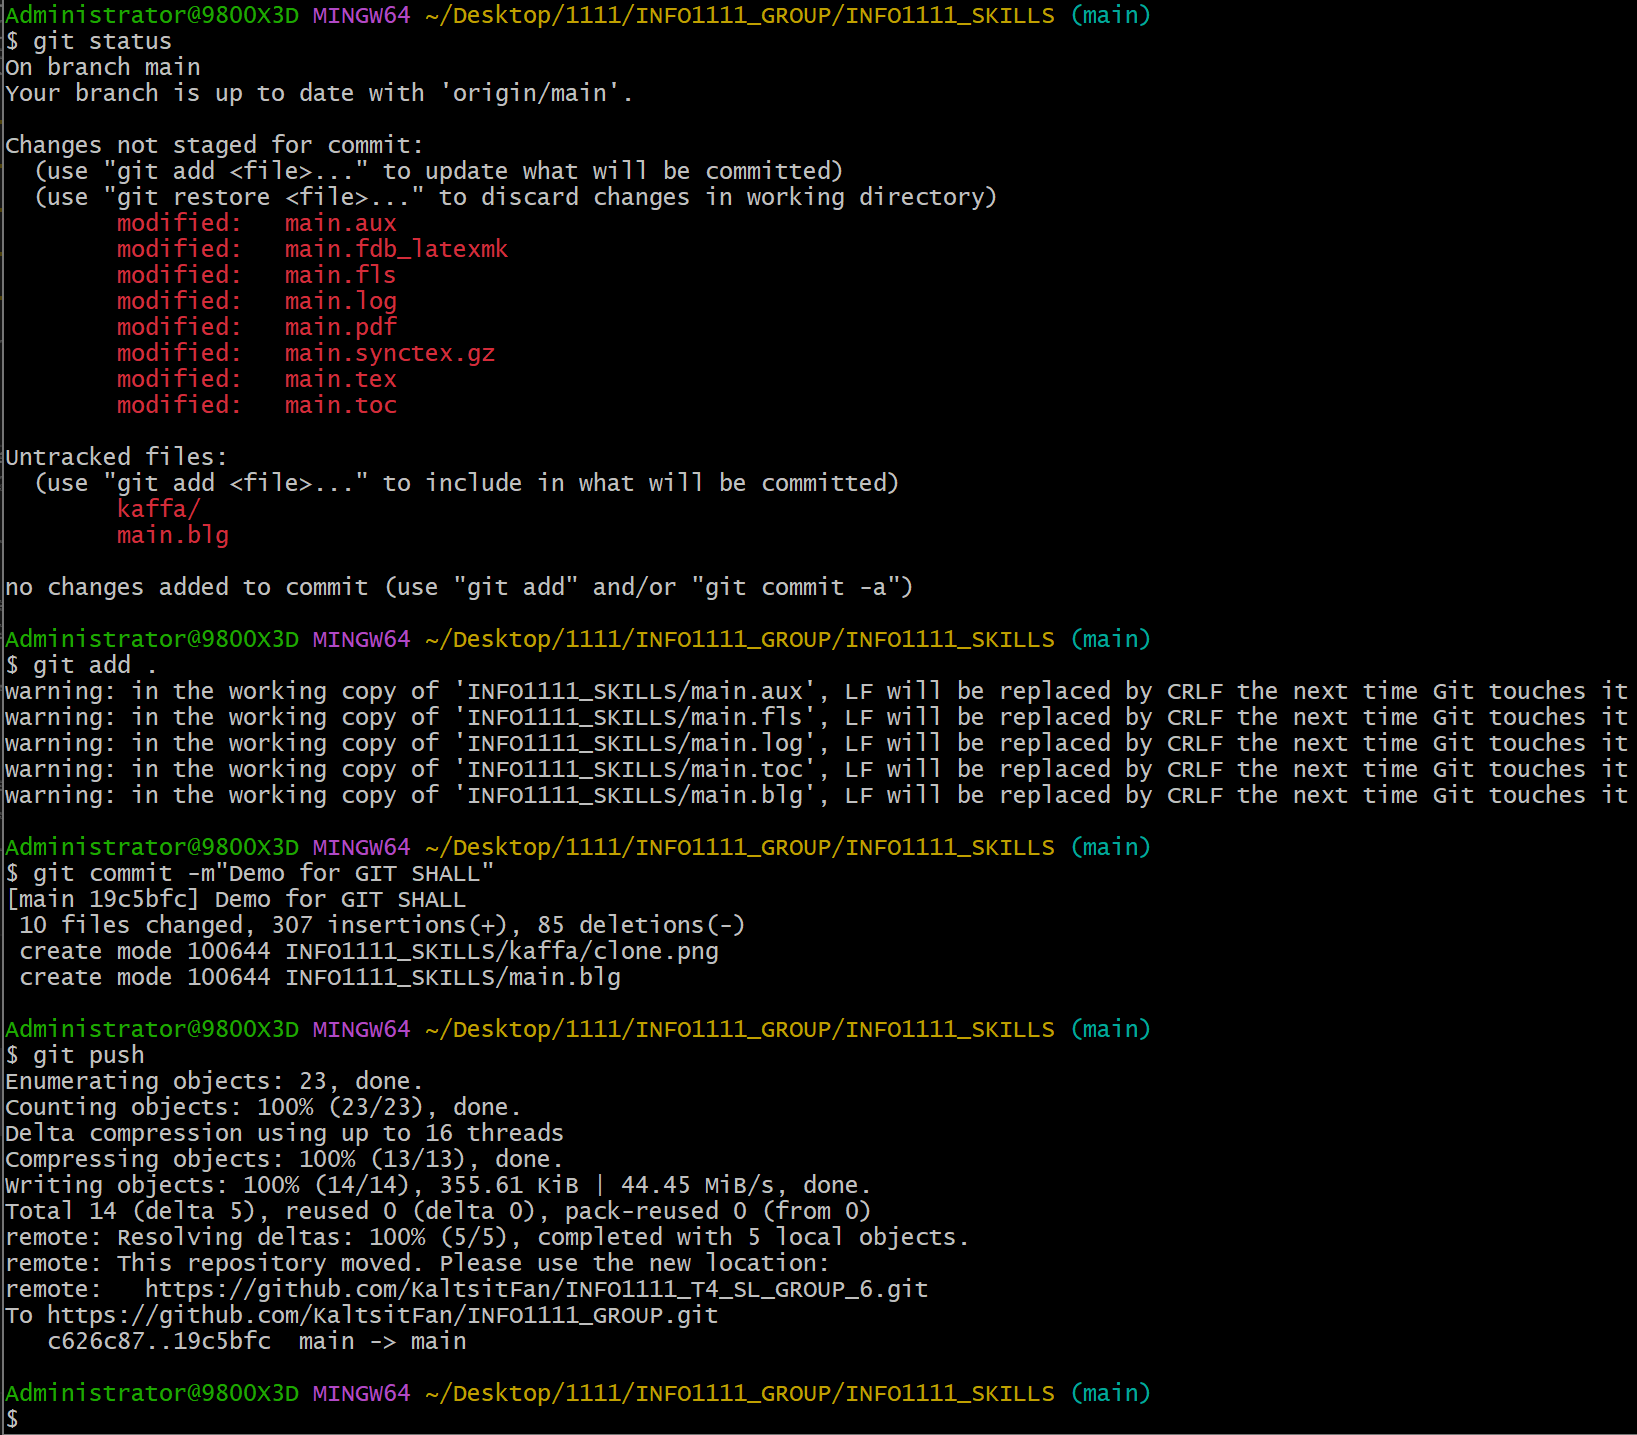
\includegraphics[width=0.8\textwidth]{kaffa/push.png}
\captionof{figure}{Adding files to the staging area}
\end{center}

\textbf{3.synchronization}
\begin{verbatim}
git add .
\end{verbatim}
Stage all modified files to prepare them for commit.

\begin{center}
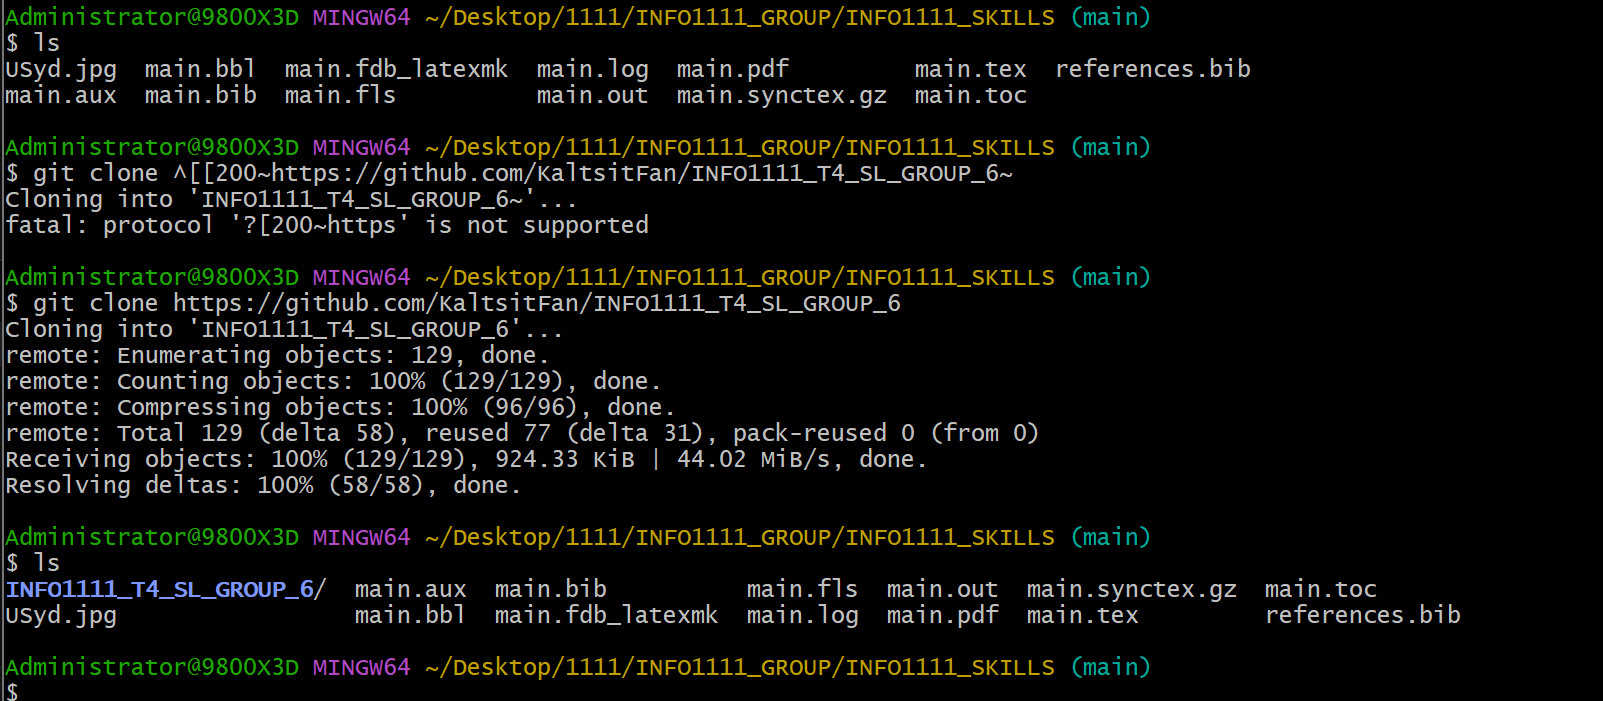
\includegraphics[width=0.8\textwidth]{kaffa/clone.png}
\captionof{figure}{Adding files to the staging area}
\end{center}




\newpage

\subsection{Skills for SW Development: Jared Song}
Through this project, I identified two critical skills from the SFIA framework relevant to software development:

\subsubsection{Key Technical Skills}
\begin{itemize}
    \item \textbf{PROG (Programming/Software Development)} \\
    According to the SFIA framework~\cite{sfia}, developing the disaster system's offline functionality required:
    \begin{itemize}
        \item Implementing local data caching using Python's \texttt{shelve} module
        \item Writing thread-safe code for concurrent access during emergencies
    \end{itemize}

    \item \textbf{TEST (Software Testing)} \\
    Establish comprehensive test coverage for disaster scenarios:
    \begin{itemize}
        \item Parameterized test suite covering distinct failure modes:
        \begin{itemize}
            \item Network partitions (simulated with \texttt{pytest-timeout})
            \item Data corruption (CRC32 validation tests)
            \item Resource exhaustion (memory/stress tests)
        \end{itemize}

        \item Mock service framework featuring:
        \begin{itemize}
            \item Configurable failure injection 
            \item Latency simulation 
            \item Stateful behavior modeling
        \end{itemize}
    \end{itemize}
\end{itemize}

\subsubsection{Skill Development through Collaboration}
According to the SFIA framework~\cite{sfia}, The team environment enhanced these skills by:
\begin{itemize}
    \item \textbf{Cross-domain feedback}: Data Science members' statistical analysis helped refine our cache invalidation algorithm, the data collected has also simplified the work and made the work more straightforward.
    \item \textbf{Collective problem-solving}: Pair programming sessions fixed race conditions in the resource allocator module
    \item \textbf{Tool knowledge sharing}: Learned GitHub Actions CI configuration from Computer Science teammate, which really helps me enhance my skills and understanding of GitHub.
\end{itemize}

\subsubsection{Areas for Improvement}  
Through my work on the disaster response system, I've identified several technical and professional skills that require refinement:
\begin{itemize}
    \item \textbf{Performance Optimization}: Need deeper understanding of profiling tools (e.g. cProfile) - evidenced when our stress tests failed at 10,000+ concurrent users, be able to learn more about Python and be proficient in using Python. 
    \item \textbf{Technical Documentation}: Find difficulty in using Github and Latex, so learning more skills and implementing automated documentation generation are important.
\end{itemize}   

\subsection{Skills for Cybersecurity: Barnett Zheng}
Through this project, I identified two critical skills from the SFIA framework relevant to cybersecurity:

\subsubsection{Key Technical Skills}
\begin{itemize}
    \item \textbf{SCTY (Network Security)} \\
    Securing communication channels in the disaster response system required:
    \begin{itemize}
        \item Implementing firewall rules to restrict unauthorized access
        \item Encrypting data transmissions using TLS to ensure confidentiality
        \item Deploying intrusion detection systems (IDS) to monitor for suspicious activity
    \end{itemize}

    \item \textbf{SCTY (Data Protection)} \\
    Ensuring the privacy and integrity of user data involved:
    \begin{itemize}
        \item Utilizing AES encryption for sensitive personal information storage
        \item Implementing access controls to restrict unauthorized data retrieval
        \item Performing regular security audits to detect vulnerabilities
    \end{itemize}
\end{itemize}

\subsubsection{Skill Development through Collaboration}
The team environment enhanced these cybersecurity skills by:
\begin{itemize}
    \item \textbf{Interdisciplinary Insights}: Working with software engineers helped me align security mechanisms with application logic, ensuring seamless integration.
    \item \textbf{Incident Response Drills}: Collaborating with the team in security simulations improved my ability to detect and mitigate threats quickly.
    \item \textbf{Knowledge Sharing}: Gained practical experience with GitHub security features, such as dependency scanning and secret detection.
\end{itemize}

\subsubsection{Areas for Improvement}  
Through my work on the disaster response system, I've identified several cybersecurity skills that require further refinement:
\begin{itemize}
    \item \textbf{USUP (Incident Response)}: Need to enhance my ability to analyze and react to security breaches in real time, particularly in high-pressure situations.
    \item \textbf{RESL (Risk Assessment)}: Improve my ability to evaluate and prioritize security threats, ensuring that mitigation efforts focus on the most critical risks.
\end{itemize}   

\subsection*{Skills for Data Science: Link Lin}

Through my work exploring data science applications, particularly in disaster response and predictive analytics, I identified two critical skills relevant to data science based on their practical importance:

\subsubsection*{Key Technical Skills}
\begin{itemize}
    \item \textbf{Data Integration} \\
    Effective data integration for disaster scenarios required:
    \begin{itemize}
        \item Combining diverse datasets (e.g., satellite imagery, weather forecasts) using Python’s \texttt{Pandas} library
        \item Normalizing inconsistent formats for real-time visualization during emergencies
    \end{itemize}

    \item \textbf{Predictive Modeling} \\
    Building robust predictive models for fire prevention involved:
    \begin{itemize}
        \item Analyzing historical weather and topographic data with:
        \begin{itemize}
            \item Machine learning algorithms (e.g., Random Forests)
            \item Cross-validation to prevent overfitting
        \end{itemize}
        \item Simulating fire spread scenarios featuring:
        \begin{itemize}
            \item Temperature and humidity forecasting
            \item Wind speed impact modeling
            \item Risk area prioritization
        \end{itemize}
    \end{itemize}
\end{itemize}

\subsubsection*{Skill Development through Collaboration}
The team environment enhanced these skills by:
\begin{itemize}
    \item \textbf{Cross-disciplinary input}: Feedback from software development teammates improved data pipeline efficiency, optimizing how integrated data fed into predictive models.
    \item \textbf{Group troubleshooting}: Collaborative debugging sessions refined model accuracy by addressing data preprocessing errors.
    \item \textbf{Tool adoption}: Learned Jupyter Notebook workflows from a teammate, enhancing my ability to prototype and visualize data integration outputs.
\end{itemize}

\subsubsection*{Areas for Improvement}
Through my data science efforts, I’ve identified key areas for growth:
\begin{itemize}
    \item \textbf{Data Quality Handling}: Need better proficiency in manual data cleaning techniques (e.g., handling missing values), as shown when inconsistent weather data skewed early predictions.
    \item \textbf{Model Interpretability}: Struggle to explain complex model outputs clearly; improving visualization skills with tools like Matplotlib or Seaborn will aid communication with non-technical stakeholders.
\end{itemize}


\newpage

\section{Submission contribution overview}

For each submission, outline the approach taken to your teamwork, how you combined the various contributions, and whether there were any significant variations in the levels of involvement. (Target = $\sim$100-300 words).

\subsection{Submission 1 contribution overview}

As above, for submission 1

\subsection{Submission 2 contribution overview}

As above, for submission 2

\subsection{Submission 3 contribution overview}

As above, for submission 3


%=======================================================================================

\newpage

\bibliographystyle{IEEEtran}
\bibliography{main}

\end{document}
\end{report}
